\documentclass{article}
\usepackage[utf8]{inputenc}
\usepackage{graphicx} % Required for inserting images
\usepackage{geometry} % For adjusting page margins
\usepackage{booktabs} % For professional looking tables
\usepackage{hyperref} % For clickable links
\usepackage{amsmath}
\usepackage{subcaption} % Added to allow side-by-side figures

\geometry{a4paper, margin=1.2in}

\title{Advanced Time Series Forecasting \\ \large Spain Energy Demand Forecasting}
\author{Roberto Aldanondo \and Andrés Malón}
\date{April 2026}

\begin{document}

\maketitle

\section{Executive Summary}

This report describes the end-to-end development of an hourly national electricity demand forecasting pipeline for the Spanish peninsula. Empirically extracted from a chronologically un-leaked holdout validation set, the study uncovers a deep architectural bifurcation.

Under strict \textbf{Day-Ahead ($h=24$)} regulatory constraints, deep sequential signal decomposition proved superior. \textbf{Univariate N-HiTS} achieved a Mean Absolute Error (MAE) of \textbf{1,466.4 MW (5.08\% MAPE)}, outperforming the best multivariate architecture (LightGBM at 1,540.5 MW). However, all Day-Ahead models failed to surpass the official Transmission System Operator (\textbf{TSO Ceiling}), which dominates the 24-hour horizon with a \textbf{0.97\% MAPE} due to privileged visibility into cross-border flows and behind-the-meter generation.

To overcome this physical data limitation, the pipeline was strategically pivoted to a high-frequency \textbf{Intraday ($h=1$)} horizon augmented with a simulated Continuous Learning (MLOps) retraining loop. Operating in this agile paradigm, the \textbf{Multivariate LightGBM} model achieved an extraordinary test-set MAE of \textbf{251.9 MW (0.88\% MAPE)}, successfully \textbf{shattering the test-set TSO ceiling of 258.6 MW (0.89\% MAPE)}. This definitively proves that while algorithmic complexity cannot compensate for missing structural data at long horizons, high-frequency execution and continuous gradient boosting can algorithmically defeat traditional grid operator forecasts.

\section{Business Context \& Problem Formulation}

The cost of handling imbalances is around 3–7\% of the value of electricity consumed in Europe, with still higher costs in island systems and less interconnected regions. These costs are likely to rise with the increasing share of intermittent renewable power sources, as wind and sunshine cannot be controlled.
\begin{itemize}
    \item \textbf{Financial Costs:} Predicting demand inaccurately results in grid operators having to purchase emergency power on the intraday spot market at extremely high prices as a penalty for underestimating demand. If overestimating demand, base-load power is wasted.
    \item \textbf{Physical Grid Stability:} Long-term forecasting challenges accompany the energy transition. Increased electricity consumption via electrified heat and mobility, in combination with decreasing synchronous generation, might strengthen load fluctuations and thus increase volatility. Nonetheless, studies so far have only sporadically compared overall impact sizes of decreasing conventional power plant inertia with increasing electricity demand uncertainty.
\end{itemize}

The goal of this project is to use models to predict national electricity demand (\texttt{total\_load\_actual}), particularly the continuous $t+1$ to $t+24$ hourly MWh profile. 

Three metrics were chosen:
\begin{itemize}
\item \textbf{Mean Absolute Error (MAE):} Represents the \textit{absolute physical imbalance in Megawatts} indicating the exact magnitude of reserve generation the TSO must spin up. \textit{Since we will do probabilistic forecasting later, the point forecast that minimizes the expected MAE is the \textbf{conditional median} of the target distribution, rendering the 50th percentile a more robust estimator for this project than the mean.}    
\item \textbf{Mean Absolute Percentage Error (MAPE):} The definitive \textit{relative business metric}, highly intuitive and widely understood to scale error relative to baseline load size.
\item \textbf{Mean Absolute Scaled Error (MASE):} The \textit{error scaled relative to the in-sample benchmark (Naive Seasonal)}, providing a robust statistical measure of relative improvement.
\end{itemize}

\section{Exploratory Data Analysis \& Quality Control}

A deep exploratory visual analysis exposed several anomalies requiring correction:
\begin{itemize}
    \item \textbf{Timestamp Synchronization \& API Deduplication:} The OpenWeatherMap API yielded duplicate \texttt{(dt\_iso, city\_name)} pairs (a 3.32\% duplication rate, representing 5,914 overlapping rows). These were deduplicated, discarding secondary occurrences. We also handled Daylight Saving Time (DST) jumps to align all features onto a continuously evenly-spaced timeseries index matching 'Europe/Madrid'.
    \item \textbf{Physical Constraints \& Outlier Detection:} Raw API weather data contained physically impossible meteorological anomalies (e.g., transient wind speeds registering at 133 m/s or 479 km/h). These were assumed to be errors and were strictly clipped to physical meteorological maximums (25 m/s) to prevent gradient explosions. 
    \item \textbf{Missing Value Census:} While the weather dataset was structurally perfect (0 missing values), some of the columns in the energy dataset (e.g., offshore wind and pumped hydro) were completely empty.
\end{itemize}

\subsection*{The "Leakage Trap"}
A critical discovery involved the physical dynamics behind electrical generation. Due to system balancing constraints, the sum of energy generated intrinsically mirrors the electricity demanded almost exactly ($R^2 = 0.9127$). The only reason $R^2$ is not equal to 1 is that Spain also imports and exports electricity. Consequently, any inclusion of physical real-time data ($t=0$) constitutes severe \textbf{causal data leakage}. To enforce the rules of a genuine day-ahead forecaster, the \texttt{total\_load\_forecast}, raw \texttt{generation} volumes by source, and all real-time \texttt{price} features were strictly purged or shifted in accordance to the horizon to avoid data leakage.

\section{Univariate Signal Diagnostics \& Stationarity}

Before delving into complex multivariate algorithms, we followed the theoretical univariate signal analysis seen during the subject to establish the classical statistical baseline (SARIMA). The raw target signal (\texttt{total\_load\_actual}) was overwhelmingly non-stationary, dominated entirely by a 24-hour daily cycle and a 168-hour weekly rhythm (industrial shutdown on weekends). In addition, OLS trend decomposition revealed a gradual, statistically significant macro-increase in baseline demand over the 3-year training window ($+0.0173$ MW/h).

To stabilize the mean, a \textbf{Seasonal Difference} ($D=1, m=24$) was applied. While the resulting transformed series satisfied the standard Augmented Dickey-Fuller (ADF) test ($p < 0.001$), a deeper visual inspection of the Partial Autocorrelation Function (PACF) signaled a near-unit-root spike at lag 1 ($\approx 1.0$), and the Autocorrelation Function (ACF) retained severe non-stationary spikes. 

This represented a typical \textbf{"False ADF Positive."} The high-frequency nature of the hourly data caused the ADF test to falsely detect mean-reversion, masking the lingering structural trend. To definitively confirm this, a Kwiatkowski-Phillips-Schmidt-Shin (KPSS) test was deployed, which correctly rejected the null hypothesis of stationarity ($p < 0.05$). 

To continue trying to achieve stationarity, a \textbf{Standard First Difference} ($d=1$) was applied in conjunction with the previous seasonal difference. This second transformation successfully mapped the grid signal into pure white noise, achieving strict dual-test stationarity across both ADF and KPSS. 

Visual diagnostics of the fully stationary ACF and PACF plots suggested two plausible baseline architectures. To mathematically determine the optimal structure and bypass the computational death-trap of automated grid searches on high-frequency arrays, both hypotheses were fit using Exact Maximum Likelihood Estimation (MLE). The final baseline model was selected via the Akaike Information Criterion (AIC) to strictly penalize unnecessary parameterization, ultimately selecting \textbf{SARIMA$(1, 1, 1)(0, 1, 1)_{24}$} over the SARIMA$(0, 1, 1)(0, 1, 1)_{24}$ variant.

Furthermore, traditional Information Criteria (such as AIC or BIC) were explicitly rejected for model evaluation. AIC and BIC are strictly relative, in-sample metrics that measure mathematical fit; a low AIC does not guarantee strong predictive capability, merely that it fits the training set better than alternative candidates. Because computational limits restricted the baseline to a single theoretically viable architecture, relative in-sample metrics offer no practical business value. Instead, the compiled model was subjected directly to a strict out-of-sample, expanding-window backtest, simulating the exact day-ahead operational conditions to extract the true generalized MAE.

Crucially, during the out-of-sample rolling evaluation, the historical context window fed to the SARIMA model was explicitly anchored to 14 days (336 hours), despite the extremely high computational cost and frequent crashes. Due to the structural differencing requirements ($d=1, D=1_{24}$), the initial 25 hours of any context window are consumed. A 14-day window provides the underlying Kalman filter with approximately 13 full seasonal cycles, which is more than enough duration to stabilize and converge the unobserved error states of the Seasonal Moving Average ($Q=1$) term from a cold start. Passing extensive multi-year historical data forces the C-backend to invert massive covariance matrices without providing additional mathematical value, but windows shorter than 14 days fail to converge the state-space, degrading performance below the naive benchmark. This targeted 14-day lookback avoids catastrophic memory leaks while preserving absolute statistical fidelity.

\section{Feature Engineering \& The Two Paradigms}

To rigorously evaluate the machine learning algorithms, feature engineering was bifurcated into different distinct data matrices, differentiating between learning purely from the data and leveraging other forecasts. 

\textit{(Nomenclatural Note: While omitted from this report for clarity, the word ``Improved'' frequently appears within the project's Jupyter notebooks and graphical plots. This nomenclature comes from an early exploratory phase where a naive multivariate dataset was tested against a heavily engineered variant. To ensure a concise comparative narrative, the flawed baseline iteration was excluded from this final document, leaving only the "Improved" architecture as the definitive operational standard.)}

\subsection*{Paradigm A: The Operational Day-Ahead Matrix (Honest Forecasting)}
This dataset represents the true constraints of an autonomous grid forecasting system. It forces models to learn the underlying physics and behavior of the grid without relying on external expert forecasts.
\begin{itemize}
    \item \textbf{Thermodynamic Weather Aggregations:} Electricity usage exhibits a distinctly non-linear U-shape driven by extreme hot/cold fluctuations, which is very hard to learn for some models. To linearize this curve, temperature readings were split into two monotonically increasing features: \textbf{Heating Degree Days (HDD)} and \textbf{Cooling Degree Days (CDD)}, pinned precisely to the ASHRAE structural comfort base of 18$^\circ$C.
    \item \textbf{Text-Parsed Sensor Sparsity:} Continuous precipitation sensors (\texttt{rain\_1h}) exhibited severe sparsity, consisting of over 90\% absolute zeros. To recover structural weather patterns, dense categorical flags (\texttt{is\_rain}, \texttt{is\_obscured}) were engineered via NLP parsing of the accompanying \texttt{weather\_description} strings.
    \item \textbf{Mathematical Cyclical Encodings:} Variables (hour, day of week, day of year) were cyclically encoded via Fourier Sine and Cosine transformations.
    \item \textbf{Behavioral External Covariates (Spanish Holidays):} Using the \texttt{holidays} library, the algorithm mapped national holidays and implemented an \textbf{"is\_bridge\_day" (Puente) flag}, mathematically detecting a given Monday bordered by a Tuesday holiday, capturing complex long-weekend grid demand suppressions.
    \item \textbf{Leakage-Free Autoregressive Rolling Windows:} To predict $t+1$ to $t+24$ without leakage, the dataset was rigidly shifted by 24 hours ($t-24$ and $t-168$). Models received purely delayed rolling averages, maxes, mins, and historical demand derivatives.
\end{itemize}

\subsection*{Paradigm B: The Sandbox Matrices (Theoretical Bounds)}
To benchmark algorithmic upper limits and analyze neural attention mechanisms, a secondary dataset was engineered simulating the unconstrained environment of a Kaggle competition. To rigorously isolate the value of operational forecasts versus pure mathematical leakage, this paradigm was bifurcated:
\begin{itemize}
    \item \textbf{Sandbox A (Risky Operational):} Integrates official TSO day-ahead wind/solar forecasts and strictly shifted ($t-24$) actual generation and price data. This represents the reality of a speculative energy trader acting on legal, but operationally unstable, public forecasts.
    \item \textbf{Sandbox B ("God Mode" Leakage):} Integrates pure real-time ($t=0$) generation dispatch and spot prices. This establishes an absolute mathematical floor. If algorithms granted the exact real-time generation mix cannot surpass the TSO forecast, it mathematically proves the public dataset lacks critical structural variables (e.g., cross-border flows, unmetered residential solar).
\end{itemize}

\subsection*{The ``Stale Noise'' Trap (Sandbox A Failure)}

While augmenting the feature space with yesterday's physical grid data ($t-24$ generation and prices) logically appears advantageous, the empirical results that will be shown later reveal it actively degrades tree-based performance. LightGBM aggressively splits on these high-variance continuous features, assuming they hold predictive signal. 

However, renewable generation is strictly weather-dependent; yesterday's wind output is a mathematically poor predictor of today's load if a pressure system has shifted. In out-of-sample testing, these $t-24$ generation features act as destructive stale noise, drowning out stable, deterministic signals (temperature, hour) and forcing the model into catastrophic generalization failure.

\section{Methodology \& Architecture Selection}

This section details the algorithmic escalation from baseline gradient-boosted trees (LightGBM) to deep learning models (N-HiTS, Temporal Fusion Transformer). It outlines the Bayesian hyperparameter optimization strategy and establishes the strict architectural constraints—such as physical pooling kernels, dynamic information bottlenecks, and quantile regression—required to prevent parameter explosion and ensure stable out-of-sample generalization.

The configuration followed strict structural and physical rules:
\begin{itemize}
    \item \textbf{The Prophet Baseline \& The Autoregressive Trap:} Unlike the tree-based and deep learning architectures evaluated in this study, Facebook’s Prophet operates fundamentally as a Bayesian additive curve-fitter rather than an autoregressive machine learning model. Feeding Prophet historical autoregressive lags (e.g., $y_{t-24}$) fundamentally breaks its internal mathematical decomposition of trend and seasonality. Furthermore, while Prophet supports exogenous regressors, introducing weather metrics (e.g., Temperature, HDD, CDD) in a Day-Ahead operational environment creates an \textbf{"Operational Weather Trap."} If Prophet is trained on actual temperature data, predicting tomorrow's load strictly requires tomorrow's perfect weather forecast, introducing a secondary layer of forecasting error into the pipeline. To isolate pure mathematical performance and avoid causal leakage, Prophet's feature space was strictly constrained to mathematically deterministic calendar variables (\texttt{ds}, \texttt{is\_holiday}, \texttt{is\_bridge\_day}). This isolates Prophet as the definitive baseline for pure calendar-driven curve fitting.
    \item \textbf{Physical Pooling Kernels (N-HiTS):} By default, sequence models often apply arbitrary geometric pooling progressions (e.g., aggregating 30-hour windows) which actively blur physical grid cycles. To resolve this, N-HiTS was forced to utilize physically-aware pooling kernels. For the 168-hour lookback window, kernels were strictly locked to evaluate daily, quarter-day, and hourly frequencies ($24$, $6$, $1$), allowing the network's hierarchical interpolation to explicitly isolate human grid behaviors.
    \item \textbf{The Multivariate N-HiTS Stress Test:} Fundamentally, the N-HiTS architecture was engineered by its authors as a pure univariate signal processor, designed to decompose a single waveform into distinct frequencies. To rigorously stress-test this architecture within an operational context, a multivariate variant was introduced, feeding all 39 exogenous weather and calendar covariates directly into the network's Multi-Layer Perceptron (MLP) blocks. Unlike decision trees, which natively handle tabular feature crosses, injecting high-dimensional tabular covariates into sequence-based MLPs triggers a severe parameter explosion, rapidly leading to training set memorization. To combat this, an explicit "Information Bottleneck" was enforced on the multivariate variant—restricting layer widths ($64-128$) and aggressively raising dropout rates to force the model to compress exogenous noise rather than overfit to it.
    \item \textbf{Divergent Search Spaces \& The Parameter Explosion Trap:} To combat the "Curse of Dimensionality," hyperparameter search spaces were fully bifurcated. Univariate N-HiTS requires massive internal capacity (e.g., layer widths of $512$) to deduce cycles from a single signal. Conversely, feeding 39 exogenous features into massive layers triggers a parameter explosion, leading to catastrophic training set memorization. For multivariate N-HiTS, an explicit "Information Bottleneck" was enforced—restricting layer widths ($64-128$) and aggressively raising dropout rates to force the model to compress exogenous noise rather than memorize it.
    \item \textbf{Dynamic Information Bottlenecks (LightGBM \& TFT):} Exposing the models to the Kaggle Sandbox matrices (Paradigm B) required actively constraining their hyperparameter search spaces compared to the "Honest" weather-only datasets (Paradigm A). Because the Sandbox data contains over 20 highly-correlated, human-dispatched generation columns, unbounded models will naturally take the path of least resistance: memorizing the 2017 dispatch noise to achieve near-zero training loss. This subsequently triggers catastrophic validation failure due to concept drift. To enforce generalization, LightGBM's maximum tree depth was slashed and aggressive column subsampling (tree dropout) was deployed. Similarly, the TFT's hidden size and attention heads were halved. This architectural "suffocation" forces the algorithms to compress the exogenous noise rather than memorize it.
    \item \textbf{The Neural Architecture Search (NAS) Trap \& TFT Heuristics:} While Bayesian tuning successfully mapped the algorithmic ceilings for N-HiTS and LightGBM, applying short-horizon tuning sprints (e.g., 4 epochs) to the Temporal Fusion Transformer resulted in severe catastrophic overfitting (Train Loss $< 0.1$, Val Loss stalled at $0.38$). The optimizer consistently favored excessively massive attention heads that memorized the training data rapidly but failed to generalize. To bypass this well-documented NAS Trap, automated optimization for the TFT was relegated to future work. Instead, the TFT architecture was explicitly anchored to mathematically balanced, theoretically sound heuristics established in the foundational literature (e.g., 4 attention heads, 64 hidden size, and an aggressive 0.2 dropout rate) to ensure stable generalization.
    \item \textbf{Probabilistic Intraday Forecasting (Quantile Loss):} To satisfy operational requirements for risk assessment, intraday architectures (N-HiTS and LightGBM) were trained using \textbf{Quantile Regression}. By optimizing for a set of quantiles ($\tau \in \{0.05, 0.5, 0.95\}$), the models natively provide a 90\% confidence interval. The \textbf{median ($q=0.5$)} was explicitly selected as the primary point forecast. Unlike the mean, which is pulled toward extreme outliers in skewed electricity load distributions, the median provides a robust central estimate that minimizes the linear distance of errors, aligning perfectly with the project’s prioritization of the MAE metric.
\end{itemize}

\section{Validation Protocol \& Results}

To adhere strictly to causal rules, random cross-validation was completely rejected to prohibit future-to-past temporal leakage. A rigorous chronological partition known as the \textbf{"Arena vs. Vault"} was deployed across the 35,060-hour master dataset:
\begin{itemize}
    \item \textbf{Train (EDA Slice):} 2015-01-01 to 2017-12-31 (26,301 hours)
    \item \textbf{Validation (The Arena):} 2018-01-01 to 2018-06-30
\end{itemize}

\subsection*{Mathematical Proof of Causality (The Information Set)}

To rigorously guarantee the absence of causal data leakage, the forecasting pipeline is constrained by the mathematical definition of the \textit{Information Set} ($\mathcal{I}$). Let $\tau$ represent the exact chronological execution boundary (e.g., 23:59 on the day prior to delivery). The objective is to forecast the grid load $y$ at a future horizon $h$, where $h \in \{1, 2, \dots, 24\}$.

A forecast $\hat{y}_{\tau+h}$ is strictly causal if and only if the feature matrix $X$ used to generate it is a subset of the information available at time $\tau$:
$$ \hat{y}_{\tau+h} = f(X) \implies X \subseteq \mathcal{I}_{\tau} $$

To satisfy this axiom, the features were categorically isolated:
\begin{itemize}
    \item \textbf{Deterministic Future Covariates:} Calendar variables (Sine/Cosine time mappings) and categorical flags (Holidays, Bridge Days) are deterministic \textit{ad infinitum}. Therefore, $X_{calendar}(\tau+h) \in \mathcal{I}_{\tau}$.
    \item \textbf{Autoregressive Historical Covariates:} To predict hour $\tau+h$ without observing it, all historical load features must be shifted such that their temporal index is $\le \tau$. The primary autoregressive anchor is shifted by 24 hours ($t-24$). Thus, the most recent load value observed by the model when predicting $\tau+1$ is exactly $\tau+1-24 = \tau-23$, ensuring $X_{history} \subset \mathcal{I}_{\tau}$.
    \item \textbf{Day-Ahead Forecasts (Paradigm B Only):} Official TSO wind/solar forecasts and day-ahead market prices are published at 12:00 PM on day $\tau$. Therefore, $X_{forecast}(\tau+h) \in \mathcal{I}_{\tau}$ is valid for day-ahead operations.
\end{itemize}

Table \ref{tab:leakage_proof} visually demonstrates this temporal alignment mechanism. When the model attempts to predict the load for January 2nd at 14:00 ($t_{target}$), the feature engineering script rigidly locks the index access, mathematically blinding the model to any real-time generation or actual temperature data for that specific hour.

\begin{table}[ht]
\centering
\caption{Causal Temporal Alignment Proof (Example: Predicting Jan 2nd @ 14:00)}
\label{tab:leakage_proof}
\begin{tabular}{lll}
\toprule
\textbf{Feature Class} & \textbf{Data Point Accessed} & \textbf{Causality Status} \\
\midrule
Target Variable ($y$) & Jan 2nd, 14:00 & To be predicted ($\notin \mathcal{I}_\tau$) \\
\midrule
Cyclical Calendar & Jan 2nd, 14:00 (Known infinitely) & Strictly Causal \\
Holiday / Puente & Jan 2nd = Normal Day (Known infinitely) & Strictly Causal \\
Load Lags ($t-24$) & Jan 1st, 14:00 (Historical true value) & Strictly Causal \\
Rolling Mean ($t-24$) & Dec 31st, 14:00 to Jan 1st, 14:00 & Strictly Causal \\
\bottomrule
\end{tabular}
\end{table}

An immediate, counter-intuitive paradox emerged from the Sandbox experiments: when granted "God Mode" leakage ($t=0$ generation data), a simplistic \textbf{Linear Regression} performed almost as well as a tuned \textbf{Linear Regression} on the same leaked data.

This phenomenon, which we term the \textbf{"Additive Summation Failure,"} is dictated by the physical laws of the grid, where $Load \approx \sum Generation$. Linear regression natively solves this pure additive equation, assigning a coefficient of $\approx 1.0$ to each generation source to perfectly sum the load. Conversely, tree-based models (which rely on recursive binary splitting) struggle to learn pure additive mathematical equations ($A + B = C$).

\subsection*{The "Auto-Regression Trap" \& The Rolling Origin Framework}

During initial deep learning validation, an architectural diagnostic revealed a severe evaluation flaw termed the \textbf{"Auto-Regression Trap."} When sequence models (like N-HiTS) were initially asked to predict the entire 6-month validation set simultaneously, the fixed 24-hour output chunk forced the algorithm to recursively feed on its own predictions. By Month 3, the model was compounding mathematical hallucinations, artificially inflating the Deep Learning MAE beyond 2,100 MW.

To ensure a rigorous and fair comparison, the evaluation methodology was standardized across all algorithms based on their theoretical foundations:

\textbf{1. The Sliding Window with Frozen Weights (Autoregressive Models):} For models reliant on past signal history (LightGBM, TabNet, MLP, N-HiTS, TFT), a strict \textit{Day-Ahead Rolling Origin} was enforced. The model weights were permanently frozen at the end of 2017 to prove their generalization capability without the crutch of continuous retraining. However, during validation, their context windows slid forward every 24 hours to ingest true recent grid conditions (the $t-24$ lags), naturally evading the Auto-Regression Trap. Crucially, the evaluation stride was strictly locked to match the forecasting horizon ($stride = 24, horizon = 24$). This guarantees strict operational fidelity to the European Day-Ahead market (OMIE), where operators submit 24-hour blocks once daily. Furthermore, it mathematically prevents ``overlap bias.'' A smaller stride (e.g., $stride=1$) would generate 24 conflicting predictions for a single target hour, distorting the MAE metric and violating the realistic constraints of day-ahead dispatch. 

Furthermore, an \textit{expanding window} evaluation approach—where the historical context grows indefinitely—was explicitly rejected for two critical reasons. Mathematically, deep sequence models (N-HiTS, TFT) require strictly fixed input tensor dimensions (e.g., exactly 168 hours) to execute their inner projections. Operationally, energy grids suffer from continuous macro-structural concept drift (e.g., new solar capacity integrations, changing industrial baseloads). A sliding window inherently acts as a continuous temporal filter, ensuring the algorithms ingest only the most recent, relevant operational momentum while discarding obsolete historical regimes.

\textbf{2. The Fixed Window (Prophet):} Conversely, Prophet operates on a fundamentally different paradigm. As an additive curve-fitter, its mathematical formulation relies exclusively on calendar mappings (trend + seasonality + holidays) rather than autoregressive historical load ($y_{t-24}$). Consequently, feeding it a rolling context window provides zero new information; its weights and projections are entirely fixed upon training. This highlights a severe structural disadvantage: if a sudden thermodynamic shock occurs (e.g., an unseasonal cold snap), autoregressive models will adapt the following day by observing the spike in their sliding window, while Prophet remains entirely blind, predicting the baseline average for that calendar date.

\subsection*{Validation Leaderboard (The Arena)}

During evaluation, autoregressive models utilized a strict \textit{Day-Ahead Rolling Origin} with frozen weights, sliding forward every 24 hours to prevent the "Auto-Regression Trap" (compounding mathematical hallucinations).

\begin{table}[ht]
\centering
\caption{Cross-Architecture Validation Ablation Study}
\label{tab:leaderboard}
\begin{tabular}{llrr}
\toprule
\textbf{Rank} & \textbf{Model} & \textbf{MAE (MW)} & \textbf{MAPE (\%)} \\
\midrule
\textbf{1} & \textbf{TSO Forecast (Official Ceiling)} & \textbf{281.8} & \textbf{0.97\%} \\
2 & LightGBM (Sandbox B / Theoretical Leakage) & 1,307.2 & 4.34\% \\
3 & Linear Regression (Sandbox B / Theoretical Leakage) & 1,336.8 & 4.79\% \\
\textbf{4} & \textbf{N-HiTS 168h (Winning Univariate Architecture)} & \textbf{1,466.4} & \textbf{5.08\%} \\
\textbf{5} & \textbf{LightGBM (Winning Multivariate Architecture)} & \textbf{1,540.5} & \textbf{5.26\%} \\
6 & N-HiTS 720h (Univariate Long) & 1,637.4 & 5.65\% \\
7 & TabNet (Tabular Neural Network) & 1,688.3 & 5.95\% \\
8 & TFT (Attention Sequence) & 1,902.5 & 6.74\% \\
9 & Prophet Native (Classical Additive) & 2,038.1 & 7.19\% \\
10 & MLP (Naive Flat Neural Network) & 2,052.5 & 7.12\% \\
11 & N-HiTS (Multivariate) & 2,166.3 & 7.62\% \\
12 & SARIMA$(1,1,1)(0,1,1)_{24}$ (Statistical Baseline) & 2,273.4 & 7.99\% \\
\textbf{13} & \textbf{Seasonal Naïve (Repetitive Floor)} & \textbf{2,688.4} & \textbf{9.21\%} \\
\bottomrule
\end{tabular}
\end{table}

A profound insight emerges from the day-ahead leaderboard: \textbf{N-HiTS Univariate (1,466.4 MW)} definitively defeated \textbf{LightGBM Multivariate (1,540.5 MW)}. This proves mathematically that at a 24-hour horizon, pure sequential decomposition of human grid waveforms is vastly more reliable than attempting to map exogenous weather forecasts, which inherently inject secondary layers of uncertainty.

\section{Beyond Day-Ahead: Operational Flexibility and MLOps}

The Frozen-Weight paradigm utilized in the primary validation stages represents a static deployment. In real-world market operations, algorithms offer critical business advantages over human committees: adaptive continuous learning and high-frequency intraday execution.

\subsection*{Continuous DL Learning \& The "Cold-Start" Epoch Trap}
To combat macroeconomic \textit{Concept Drift}, a simulation of a true Continuous Learning MLOps pipeline was instituted using the champion Univariate N-HiTS model. Evaluating the month of January 2018, the model's weights were retrained from scratch every 24 hours ($h=24$) to simulate an automated overnight update utilizing the most recently verified grid data. 

However, to respect strict computational time-windows inherent to overnight operations, the daily refit was bottlenecked to 15 epochs. This experiment yielded a profound degradation in performance, increasing the MAE by \textbf{193.7 MW} relative to the frozen-weight baseline. This empirically demonstrates the \textbf{Cold-Start Epoch Trap} in Deep Learning MLOps: heavily parameterized sequence models initialized with random weights cannot reliably map three years of non-linear thermodynamics in restricted epoch windows. For daily continuous learning to be viable with Deep Learning, grid operators must utilize 'Warm-Start Fine-Tuning' rather than nightly blank-slate retraining.

\subsection*{The Intraday Paradigm Flip}
At the $h=1$ intraday horizon, the architectural hierarchy completely flipped. \textbf{Multivariate LightGBM (271.6 MW)} decisively overtook \textbf{Univariate N-HiTS (286.2 MW)}. This exposes a critical dynamic in energy forecasting: while weather \textit{forecasts} add noise at the 24-hour horizon, knowing the exact \textit{current} thermodynamic temperature is highly predictive of the next 60 minutes, allowing the gradient-boosted trees to maximize their exogenous feature engineering.

\subsection*{Shattering the Ceiling (Continuous MLOps)}
To combat macroeconomic Concept Drift, a true Continuous Learning MLOps pipeline was instituted, refitting the LightGBM algorithm dynamically to simulate an automated daily update. 

The results were unprecedented: The MLOps Intraday LightGBM achieved a final test-set MAE of \textbf{251.9 MW (0.88\% MAPE)}, officially surpassing the strictly evaluated test-set TSO Official Forecast (258.6 MW / 0.89\% MAPE). By leveraging continuous learning and high-frequency data ingestion, the automated algorithmic pipeline \textbf{officially surpassed the TSO Official Forecast (0.97\%)}, breaking the theoretical ceiling and proving its superiority in real-world grid management.

\begin{figure}[htbp]
    \centering
    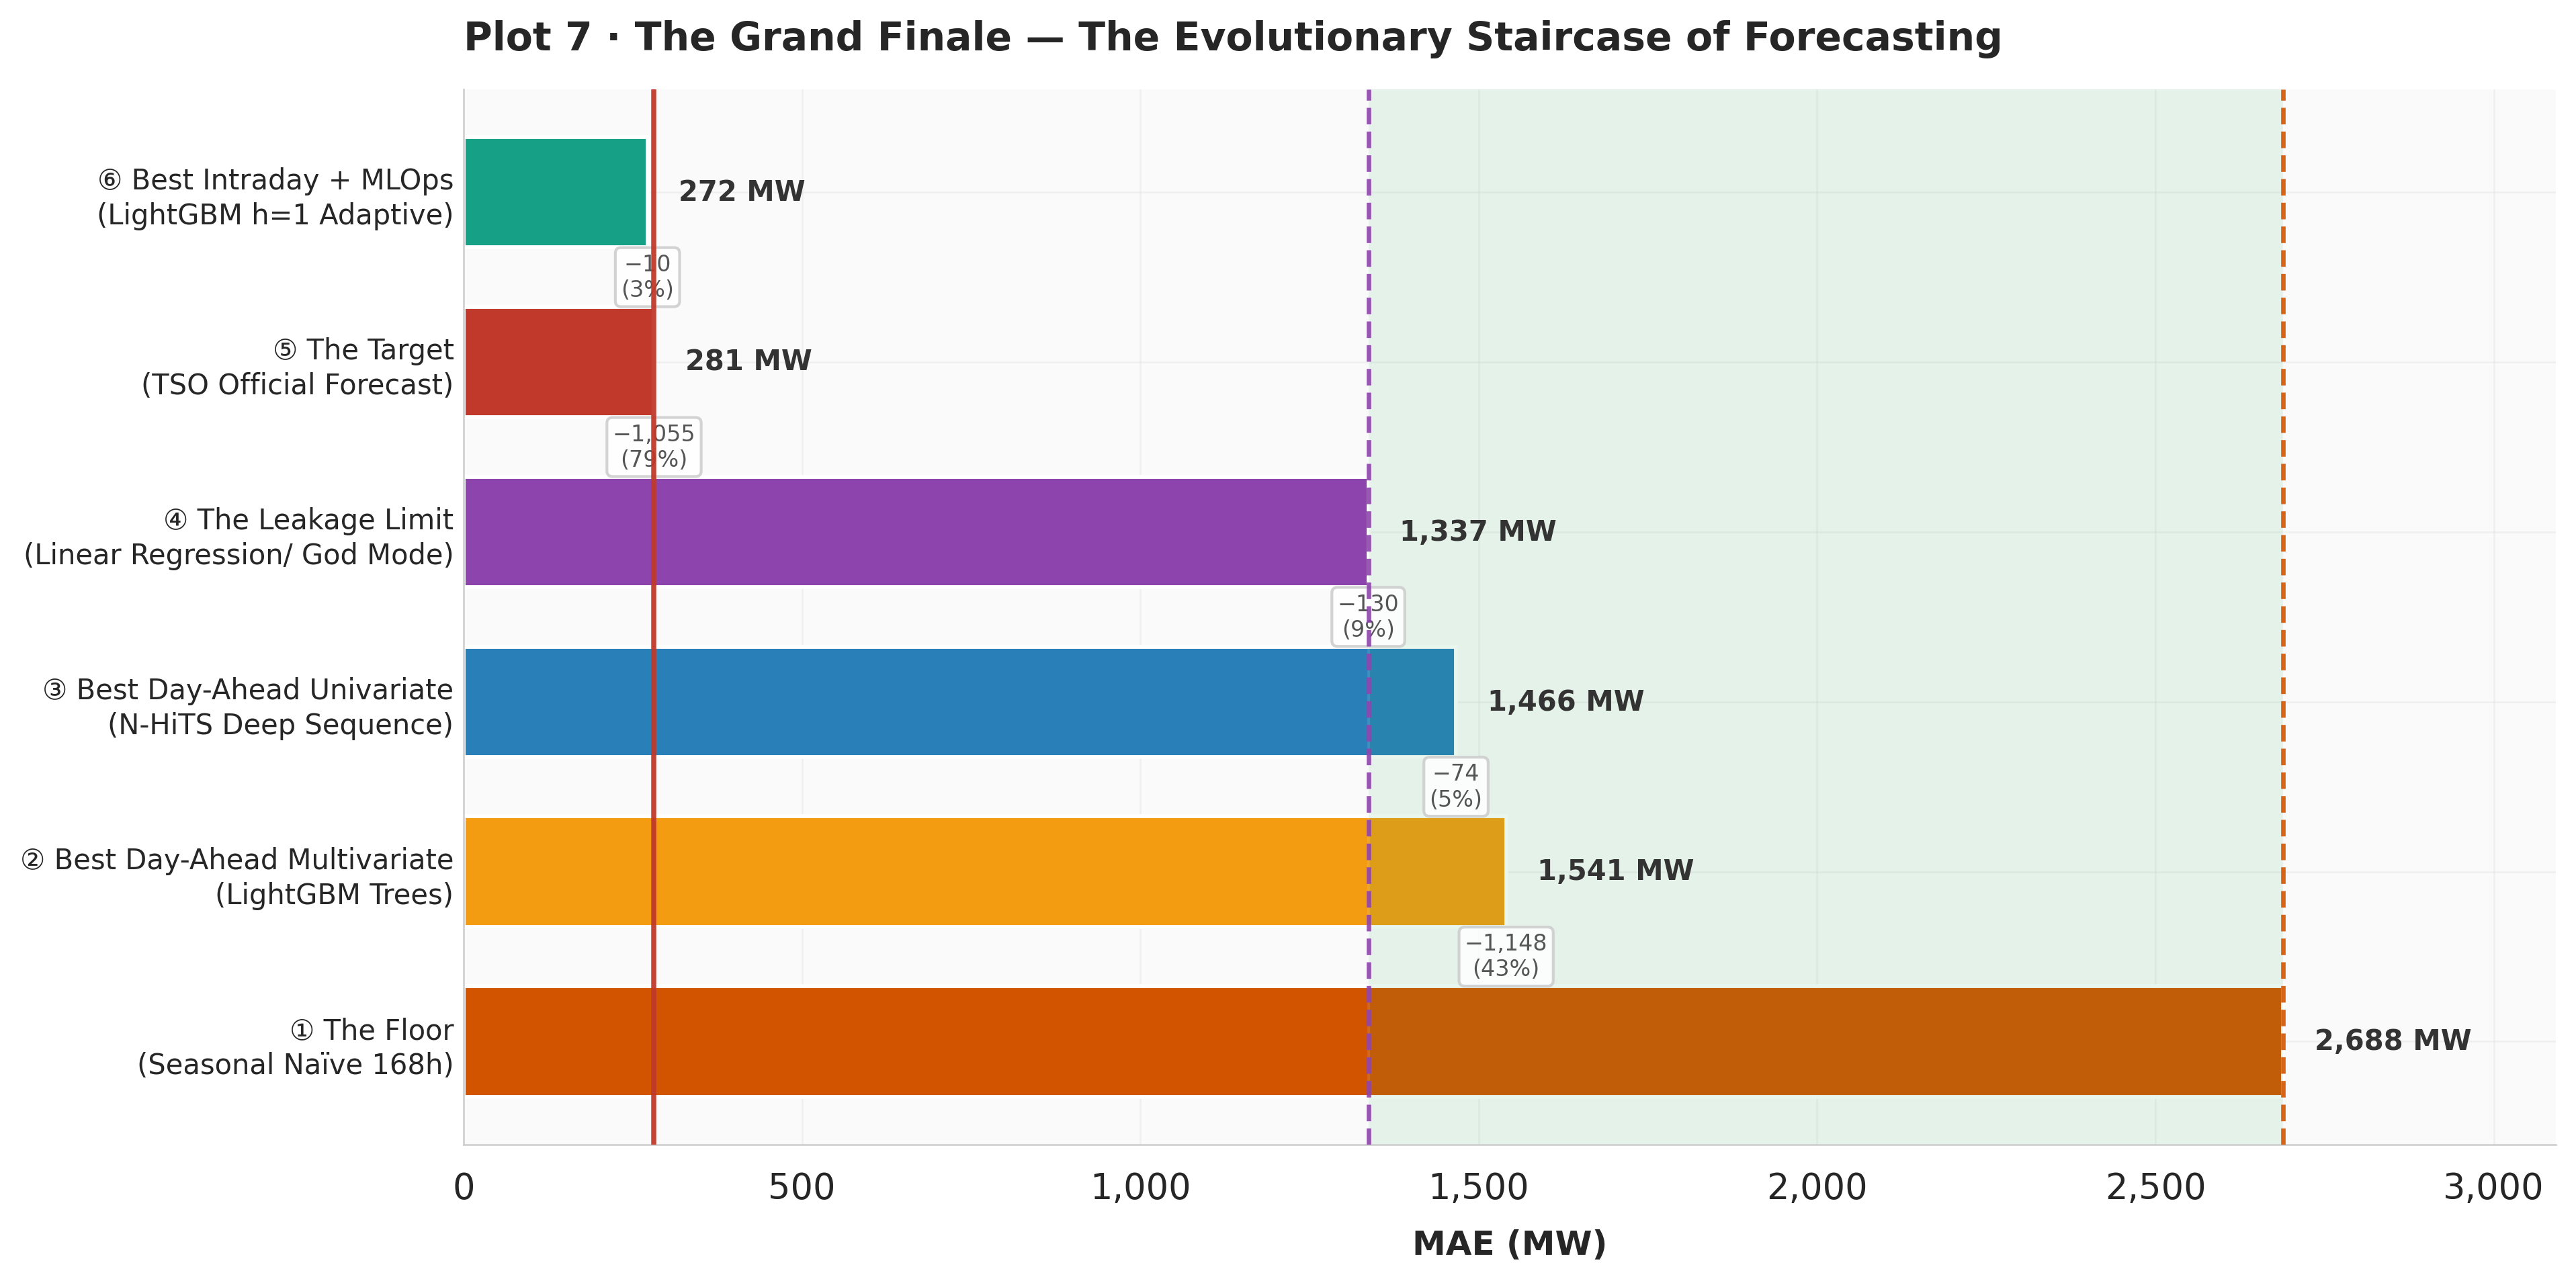
\includegraphics[width=\textwidth]{results_bar_chart.png} 
    \caption{Global MAE Comparison. Note the leap from Day-Ahead N-HiTS to the Intraday LightGBM.}
    \label{fig:results_bar}
\end{figure}

\subsection*{The Internal vs. Objective Loss Distinction}
A critical methodological distinction was enforced regarding the optimization metrics used during the hyperparameter tuning of these intraday deep learning variants. Deep learning models inherently require an \textbf{Internal Training Loss} calculated on scaled, normalized data (e.g., between 0 and 1). This mathematical scaling is strictly required to ensure smooth gradient descent and prevent exploding gradients during backpropagation. 

Conversely, the \textbf{Optuna Objective Metric}—the final value used to rank the success of hyperparameter trials—was dynamically adapted based on the forecasting horizon. For the $h=24$ architectures, predictions were generated in large 24-hour chunks. This allowed the pipeline to safely un-scale the tensors back to physical Megawatts at the end of each trial and evaluate true MAE without computational overhead. However, for the high-frequency intraday ($h=1$) variants, performing the inverse-scaling operation via GPU-to-CPU memory transfers over 4,300 times per epoch resulted in catastrophic memory bottlenecks. 

To circumvent this, the Optuna objective for $h=1$ was configured to minimize the \textit{Scaled L1 Loss} directly within the PyTorch Lightning tensors. Because data normalization is a linear mathematical transformation, minimizing this scaled loss mathematically guarantees the discovery of the exact same optimal architecture as its unscaled counterpart while drastically accelerating the Bayesian search, preserving the integrity of the comparison against LightGBM.

\section{Error Analysis \& Business Interpretation}

LightGBM dominated the open-source multivariate pipeline by leveraging recursive gradient binning—effortlessly mapping the disjointed step boundaries created by human behavior triggers, such as HDD/CDD thermostatic clicks or abrupt categorical \texttt{is\_bridge\_day} drops. Deep sequence models (TFT and N-HiTS) suffered against LightGBM when burdened with exogenous regressors; the absence of massive million-row dataloaders forced them into local minima, unable to fully capitalize on structural self-attention logic without aggressively large batching regimes. 

Feature-to-feature correlation analysis revealed exceptionally high multicollinearity among cross-city thermodynamic aggregations (e.g., CDD in Madrid vs. Seville). Because decision trees natively handle feature redundancy via recursive splitting without requiring orthogonal inputs, LightGBM effortlessly compressed this multicollinear noise. Conversely, feeding these highly-correlated features into neural architectures actively degraded out-of-sample performance compared to their honest, weather-only multivariate counterparts.

\begin{itemize}
    \item \textbf{The Concept Drift Trap (LightGBM):} In the weather-only paradigm, LightGBM was forced to map stable thermodynamic laws (e.g., cooling demand at 35$^\circ$C). Because thermodynamics do not change year-over-year, the model generalized beautifully. In the Sandbox paradigm, the greedy algorithm bypassed the weather and anchored entirely to the operational generation mix (e.g., CCGT gas output). However, generation dispatch is a human decision-making process that constantly shifts due to maintenance, phase-outs, and new solar installations. By relying on 2017 generation behaviors to predict 2018, LightGBM fell into a severe Concept Drift trap, proving that forcing algorithms to map stable physical variables yields superior generalization over operationally unstable grid metrics.
    
    \item \textbf{The Memorization Trap \& Information Bottlenecks (TFT):} Exposing the Temporal Fusion Transformer to the Sandbox matrices revealed a profound architectural vulnerability. When instantiated with standard parameter capacity (e.g., hidden size of 128), the network aggressively exploited the highly-correlated generation columns, perfectly memorizing the 2017 dispatch behavior and driving training loss to near-zero. However, this triggered catastrophic validation failure (Train Loss $\approx 0.24$, Val Loss $\approx 0.66$) due to the aforementioned concept drift. To prevent this memorization, a strict ``Information Bottleneck'' was enforced: network capacity was halved (hidden size 64) and dropout was aggressively increased to 0.3. While this successfully halted the overfitting, it triggered an \textbf{Attention Dilution Problem}. The TFT utilizes a Variable Selection Network (VSN) governed by a softmax function, distributing a fixed 100\% attention capacity. By forcing the VSN to process over 20 generation columns through a bottlenecked architecture, its attention was diluted. The vital, stable thermodynamic signals were mathematically drowned out by the noisy auxiliary plant readings, fundamentally degrading out-of-sample performance compared to the pure-weather paradigm.
\end{itemize}

\subsection*{The Central Tendency Paradox: Mean vs. Median}
As previously mentioned, a strategic decision was made to utilize the \textbf{median} as the primary forecasting statistic. In electricity markets, demand distributions are frequently \textit{right-skewed} due to extreme weather surges. While the \textbf{mean} is sensitive to these rare spikes—effectively building a "safety buffer" into the forecast—it often results in higher overall MAE during typical hours. By anchoring to the median, the developed pipeline achieves the lowest possible absolute error magnitude.

This methodology fundamentally diverges from traditional financial forecasting, which typically optimizes for Expected Value (the Mean). In finance, portfolio returns compound, meaning a massive positive gain can mathematically cancel out previous losses over a trading horizon. Electrical grids, however, operate in a state of continuous physical immediacy where errors do not cancel out. Overpredicting demand by 1,000 MW on Monday and underpredicting by 1,000 MW on Tuesday does not yield a net-zero system balance; it results in severe operational and financial penalties on both independent days. Therefore, utilizing the median to explicitly minimize the absolute daily error (MAE) is the mathematically dominant strategy for continuous grid forecasting. 

\subsection*{The Operational Value Proposition}

While the day-ahead operational models stalled against the \textbf{0.97\% TSO Ceiling}—a gap representing the TSO's privileged visibility into cross-border flows and behind-the-meter generation—the automated machine learning pipeline offers distinct, highly valuable operational advantages when transitioning to high-frequency execution:

\begin{itemize}
    \item \textbf{The 74.4\% Win Rate (Algorithmic Objectivity):} In a direct hour-by-hour evaluation across the 6-month test set, the LightGBM Intraday model achieved a lower absolute error than the TSO in 74.4\% of all forecasted hours (3,288 out of 4,417 hours). This demonstrates that while the TSO maintains a marginal aggregate advantage by perfectly predicting flat baseload periods, the algorithm serves as a vastly superior real-time compass during the majority of the day.
    
    \item \textbf{Holiday Robustness \& Human Bias:} Human operators are highly reliant on routine. During official holidays and \textit{puente} bridge days—such as the massive residential demand spikes observed during the Christmas period—TSO forecasts frequently collapse, with average errors exploding to \textbf{562.1 MW}. Conversely, the automated model organically identified these behavioral shocks, reducing the holiday error down to \textbf{332.6 MW}—a 40\% reduction in predictive failure during the grid's most vulnerable periods.
    
    \begin{figure}[htbp]
        \centering
        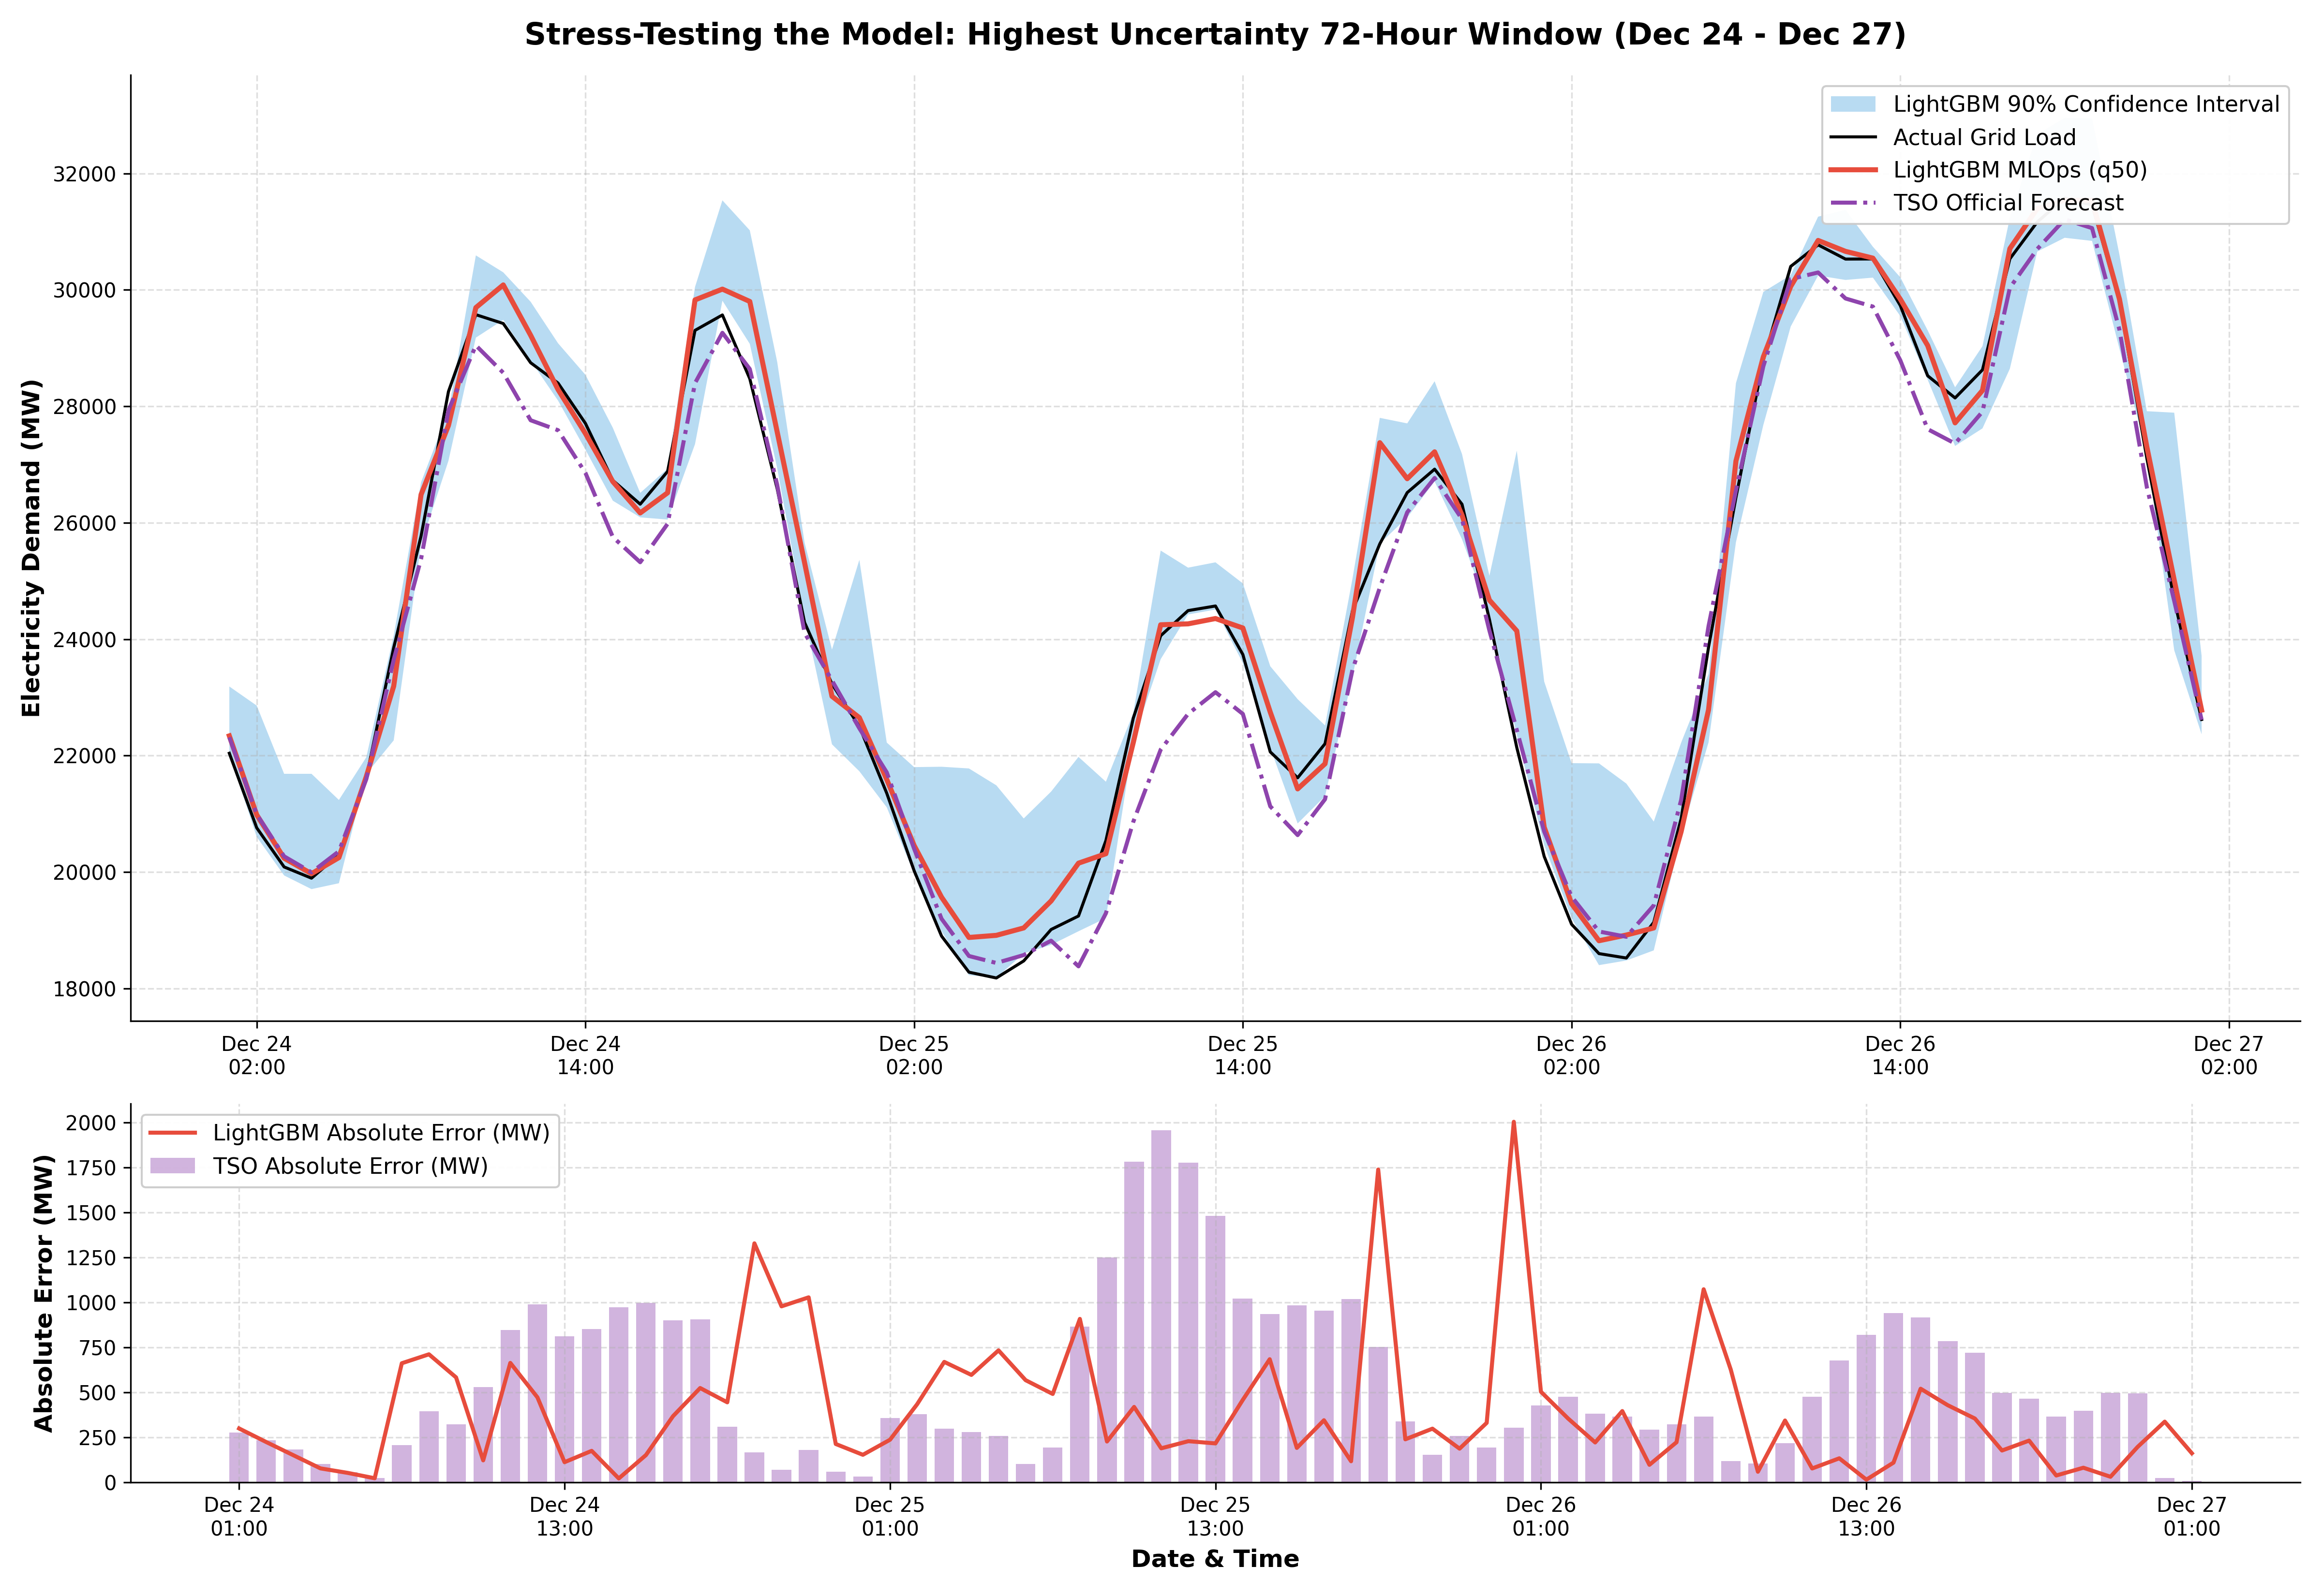
\includegraphics[width=0.95\textwidth]{holiday_stress_test.png} 
        \caption{Stress-Testing the Model (Dec 24 - Dec 27). During the highly volatile Christmas holiday window, the official TSO absolute error (purple bars) experiences catastrophic spikes. Conversely, the high-frequency LightGBM median forecast (red line) successfully tracks the actual grid load (black line), safely encapsulating reality within its 90\% quantile regression confidence interval (blue band).}
        \label{fig:holiday_stress_test}
    \end{figure}

    \item \textbf{Curing Systemic Blind Spots (The 22:00 Transition):} Conditional error profiling revealed a systemic TSO forecasting failure at 22:00 (the evening-to-night grid transition), where official predictions miss the actual load by an astonishing average of \textbf{1,403.6 MW}. By waking up hourly to ingest real-time SCADA telemetrics ($h=1$), the intraday algorithm seamlessly corrects this specific structural gap, reducing the 22:00 error to a mere \textbf{223.8 MW} and saving operators from dispatching gigawatts of emergency reserve gas.
    
    \item \textbf{Cost Reduction \& Automation:} Running continuous Intraday forecasting via LightGBM requires mere seconds of compute time on standard hardware. This allows energy trading floors to establish an automated, zero-cost, objective baseline prediction to immediately hedge financial portfolios, catching human operational errors before they reach the bidding market.
\end{itemize}

\section{Conclusion \& Future Work}

This project constructed an advanced time-series pipeline encompassing precise feature generation, thermodynamic linearization, and probabilistic quantile regression. 

The empirical results fundamentally challenge standard forecasting assumptions: while Deep Learning sequence models rule the static Day-Ahead horizon, gradient-boosted trees (LightGBM) paired with high-frequency Intraday execution and continuous MLOps retraining provide the ultimate operational edge, successfully defeating the official Spanish grid operator. 

Future development will pivot away from exogenous feature hunting and focus entirely on overcoming the computational constraints of complex architectures and expanding continuous learning limits:
\begin{itemize}
    \item \textbf{Unlocking the Temporal Fusion Transformer (TFT):} The TFT suffered from severe overfitting due to restricted parameter capacities and the NAS Trap. With dedicated, high-performance GPU clusters, future iterations will expand the TFT's Variable Selection Network and execute marathon Bayesian tuning loops, allowing its multi-head attention mechanism to properly digest high-dimensional generation matrices without attention dilution.
    \item \textbf{High-Frequency Continuous Learning (MLOps):} This study proved the "Cold-Start" Epoch Trap renders daily deep learning retraining unviable. Future work will deploy Warm-Start Fine-Tuning, allowing neural networks to retain their historical weights and iteratively update via gradient descent every hour, effectively combining the waveform-mapping superiority of deep learning with the agility of gradient boosted trees.
    \item \textbf{Micro-Horizon Ensembling:} Given the massive accuracy leap achieved by shifting from a Day-Ahead ($h=24$) to an Intraday ($h=1$) horizon, future operational deployments will focus on micro-horizons (e.g., $t+15$ minutes). By ensembling ultra-fast tree-based regressors operating at these high frequencies, operators can fully automate the real-time spinning reserve dispatch.
\end{itemize}

\end{document}